\documentclass[12pt]{article}
\usepackage[latin9]{inputenc}
\usepackage{microtype}
\usepackage[letterpaper]{geometry}
\geometry{verbose,tmargin=1in,bmargin=1in,lmargin=1in,rmargin=1in}
\pagestyle{plain}
\usepackage{color}
\usepackage{float}
\usepackage{amsmath}
\usepackage{amssymb}
\usepackage{graphicx}
\usepackage[authoryear]{natbib}
\usepackage{chngcntr}
\usepackage{subcaption}

%%%%%%%%%%%%%%%%%%%%%%%%%%%%%%  SPACING
\usepackage{setspace}

\onehalfspacing % working paper spacing

%\doublespacing % journal submission spacing
%\usepackage{footmisc} % journal submission spacing
%\renewcommand{\footnotelayout}{\doublespacing} % journal submission spacing
%%%%%%%%%%%%%%%%%%%%%%%%%%%%%% 

\usepackage{xr}
\externaldocument{AGS_Output_Subsidies}

\usepackage[unicode=true,
 bookmarks=false,
 breaklinks=false,pdfborder={0 0 1},backref=false,
 hidelinks]
 {hyperref}
\usepackage{breakurl}

\makeatletter

%%%%%%%%%%%%%%%%%%%%%%%%%%%%%%  PACKAGES FOR COMMENTING
% USER WRITTEN COMMENT COMMAND

% IF SELECTED, COMMAND WILL NOT DISPLAY COMMENTED TEXT  
%\newcommand{\comment}[1]{}  %comment not shown

%IF SELECTED, COMMAND WILL PRINT COMMENTED TEXT IN BLUE  
\newcommand{\comment}[1]
{{\bfseries \color{red} #1}} %comment shown

%%%%%%%%%%%%%%%%%%%%%%%%%%%%%% User specified LaTeX commands.
\setcounter{MaxMatrixCols}{10}

\usepackage{booktabs}% Pretty tables
\usepackage{tabularx}% 
\usepackage{threeparttable}% For Notes below table

\usepackage{amsfonts}
\usepackage{multicol}
\usepackage{lscape}
\usepackage{rotating}

\usepackage{changepage}
\usepackage{pdfpages}
\usepackage{geometry}
\usepackage{graphicx}

\usepackage{xcolor}

%PUT DATE IN MONTH-YEAR
\usepackage{datetime}
\newdateformat{monthyeardate}{%
  \monthname[\THEMONTH] \THEYEAR}
\makeatother

\begin{document}

\thispagestyle{plain}

\title{Online Appendix for: \\ Investment versus Output Subsidies: Implications of Alternative Incentives for Wind Energy}
\author{Joseph E. Aldy, Todd D. Gerarden, and Richard L. Sweeney\thanks{Aldy: Harvard Kennedy School, Resources for the Future, National Bureau of Economic Research, and Center for Strategic and International Studies (email: \href{mailto:joseph_aldy@hks.harvard.edu}{joseph\_{}aldy@hks.harvard.edu}); Gerarden: Cornell University (email: \href{mailto:gerarden@cornell.edu}{gerarden@cornell.edu}); Sweeney: Boston College (email: \href{mailto:sweeneri@bc.edu}{sweeneri@bc.edu}).}}
\date{\monthyeardate\today}

\clearpage
\maketitle
\thispagestyle{empty}

\tableofcontents


%%%%%%%%%%%%%%%%%%%%%%%%%%%%%%%%%%%% APPENDIX %%%%%%%%%%%%%%%%%%%%%%%%%%%%%%%%%%%%%%%%%%%%%%%%%%%%%%%%%%%%%%%%
\appendix

\makeatletter
\def\@seccntformat#1{\csname Pref@#1\endcsname \csname the#1\endcsname\quad}
\def\Pref@section{Appendix~}
\makeatother

\counterwithin{figure}{section}
\counterwithin{table}{section}
\counterwithin{equation}{section}


\clearpage
\section{Data Appendix \label{sec:Data_Appendix}}

\subsection{Additional Information on Data Sources and Cleaning}

Information on how to obtain each data source, along with code for replication is available on \href{https://github.com/rlsweeney/public_ags_output_subsidies}{https://github.com/rlsweeney/public\_ags\_output\_subsidies}. 

\paragraph{Additional Information on the Primary Data Sources }
\begin{itemize}
\item \href{https://www.eia.gov/electricity/data/eia860/}{Survey Form EIA-860} collects generator-specific information on an annual basis about existing and planned generators and associated environmental equipment at electric power plants with 1 megawatt or greater of combined nameplate capacity.
\item \href{https://www.eia.gov/electricity/data/eia923/}{Survey Form EIA-923} collects detailed electric power data\textemdash with both monthly and annual frequency\textemdash on electricity generation, fuel consumption, fossil fuel stocks, and receipts at the power plant and prime mover level.
\item \href{https://www.awea.org/windiq}{The American Wind Energy Association (AWEA)} collects detailed information about all of its members and makes these data available as part of its membership subscription. The database includes more than 60 fields. We use the data to determine the presence and terms of any power purchase agreements and to construct a measure of the footprint of each wind farm.
\item \href{https://www.vaisala.com/en/industries-innovation/renewable-energy-and-weather}{3TIER windspeed data} provides hourly estimated wind speed data from 2000 to 2014 for every wind farm in the EIA database. We use these hourly data to compute the variance and a polynomial in observed wind speed, as well as the potential capacity factor, for each month.\footnote{These data were provided by Joern Huenteler, Gabe Chan, Tian Tang, and Laura Diaz Anadon, collected as part of their research summarized in \citet{huenteler_why_2018}. A handful of EIA plant locations were either entered erroneously or downloaded improperly, and are excluded from the sample.}
\item \href{https://www.treasury.gov/initiatives/recovery/Pages/1603.aspx}{The Department of the Treasury} reports data on Section 1603 grant claims. We matched Treasury Section 1603 grant projects to EIA data based on business name, plant name, county and state identifiers, and date placed in service. For 152 Section 1603 grants, we could not identify a match in the EIA data. One of these is a Puerto Rico project, which is excluded due to geography from the EIA databases. The other 151 projects received very small grants, indicating that these projects were too small to be covered by EIA's EIA-860 and EIA-923 surveys. In aggregate, they represent one-half of one percent of 1603 grant outlays for large wind projects. 

A grant could be submitted for a single wind turbine, a set of turbines, or an entire wind farm. This created two data issues. First, a wind farm could receive multiple Section 1603 grants. In these cases, we aggregated 1603 grants to the wind farm level (the level of observation in the EIA databases). For example, the large Alta wind farm in California came online in phases starting in late 2010 and its developers submitted more than twenty 1603 grants. Second, a wind farm could be built with N turbines that come online before 2009, for which it claims the PTC. It may then expand with M turbines in 2009 and claim a 1603 grant for these new turbines. The EIA-observed output for that wind farm after 2009 would reflect the aggregate production of the N+M turbines. Since we cannot distinguish the output between the N PTC-claiming turbines and the M 1603 grant-claiming turbines at such a wind farm, we drop the wind farm from our sample. We identified such cases as wind farms that claimed a 1603 grant over 2009-2012, but had either substantial pre-2009 generation or a significant change in installed capacity post-2012. Using these decision rules, we dropped thirteen wind farms that represent less than four percent of total 1603 grant outlays for large wind farms. 
\end{itemize}

\paragraph*{Additional Sample Restrictions}

There are 941 wind farms in the continental U.S. in the EIA data. We restrict attention to plants that are private and operate as either independent power producers or part of an investor-owned utility based on subsidy eligibility, which reduces the sample to 817 wind farms. We also restrict the sample to plants entering before the end of the 1603 grant period (end of 2012). There are two ways of determining when a plant is placed into service using the EIA data: we could use either the date a plant submits to the EIA as their first date of commercial operation or the month that a plant's production first appears in the production data. Conversations with EIA staff confirm that the former should be used for determining 1603 grant eligibility. However, to avoid concerns about potential misclassification, we exclude plants whose two entry dates suggest conflicting 1603 eligibility status. Finally, we exclude plants that we were unable to locate in the AWEA database, plants for which we did not have site-specific wind and turbine power curve information, and plants for which the ratio of observed capacity factor to potential capacity factor was further than two standard deviations from the median. This final sample of 512 plants represents our population.

\subsection{Potential Capacity Factor Construction \label{Appendix:Potential-capacity-factor}}

As described in Section~\ref{subsec:WindEcon}, wind farm production is a nonlinear function of wind speed. This nonlinear function is turbine-specific, as some turbines are engineered to perform particularly well at low wind speeds, while others are optimized for high wind speeds. Wind turbine manufacturers provide power curves for each turbine that summarize how much electricity it should generate at a given wind speed. Figure~\ref{fig:GE-powercurve} presents example power curves for two of the most common wind turbines in the U.S. The Vestas turbine has a higher maximum capacity, but the GE turbine is rated to produce power at higher wind speeds. Other turbines are designed to generate more electricity at lower wind speeds at the expense of generating less electricity at higher speeds.

\begin{figure}[h]
\caption{Reported Power Curves for Two Common Turbines \label{fig:GE-powercurve}}
\centering{}\includegraphics[width=0.7\textwidth]{../images/powercurve_ge_vestas.png}
\end{figure}

Rather than try to approximate this function with turbine-specific high order polynomials of wind speed, we compute an ``engineering'' estimate of expected output for each turbine in each month. We begin with estimates of the wind speed every hour at every wind farm in our sample that come from 3TIER. We combine this with a location-specific power function based on the wind turbine used at each wind farm to predict hourly electricity generation. We use the ideal gas law to adjust for variation in air density, which affects the kinetic energy available to each turbine, using location- and time-specific data on temperature and pressure from 3TIER. Aggregating hourly predicted output over the month and dividing by the turbine's rated output provides us with a measure of ``potential capacity factor,'' which we include as a covariate in our primary specifications.

Table~\ref{tab:wind_selection} demonstrates that this one-dimensional, time-varying control explains significantly more of the observed variation in capacity factor than time-invariant, site-specific wind quality information. It also fits meaningully better than a third order polynomial in wind speed.

\begin{table}[H]
\caption{Explanatory Power of Alternative Measures of Potential Generation \label{tab:wind_selection}}
\footnotesize
\begin{center}
{
\def\sym#1{\ifmmode^{#1}\else\(^{#1}\)\fi}
\begin{tabular}{l*{5}{c}}
\toprule
                &\multicolumn{1}{c}{(1)}         &\multicolumn{1}{c}{(2)}         &\multicolumn{1}{c}{(3)}         &\multicolumn{1}{c}{(4)}         &\multicolumn{1}{c}{(5)}         \\
\midrule
Design Wind Speed&    0.304\sym{***}&  -0.0421         &  -0.0457         &  0.00542         &                  \\
                &  (0.104)         &  (0.106)         &  (0.105)         & (0.0908)         &                  \\
\addlinespace
Wind Speed (m/s)&                  &    0.862         &    2.163         &                  &                  \\
                &                  &  (3.470)         &  (3.527)         &                  &                  \\
\addlinespace
Wind Speed Squared&                  &    0.910\sym{**} &    0.797\sym{*}  &                  &                  \\
                &                  &  (0.418)         &  (0.419)         &                  &                  \\
\addlinespace
Wind Speed Cubed&                  &  -0.0456\sym{***}&  -0.0444\sym{***}&                  &                  \\
                &                  & (0.0151)         & (0.0150)         &                  &                  \\
\addlinespace
Var(Wind Speed) &                  &                  &    0.170         &                  &   -0.156\sym{*}  \\
                &                  &                  &  (0.136)         &                  & (0.0915)         \\
\addlinespace
Potential Capacity Factor&                  &                  &                  &    0.619\sym{***}&    0.638\sym{***}\\
                &                  &                  &                  & (0.0224)         & (0.0265)         \\
\midrule
Adjusted R-sq.  &    0.287         &    0.504         &    0.505         &    0.572         &    0.572         \\
N               &    11140         &    11140         &    11140         &    11140         &    11140         \\
\bottomrule
\end{tabular}
}

\end{center}
Results from linear regressions of observed capacity factor on functions of wind speed data from EIA and 3TIER, using data on electricity generation in 2013 and 2014 for wind farms that came online between 2005 and 2012.
\end{table}



\clearpage
\section{Negative Prices and Emissions Rates \label{Appendix:NegativePrices}}

As was discussed in Section~\ref{sec:Mechanism}, there are two possible mechanisms through which an output subsidy can increase wind production: a dispatch effect when wind is at or near the margin, and an availability effect when wind is inframarginal. Under the assumption that the true marginal cost of dispatch in any given hour is zero, the frequency of negative prices provides an upper bound on the share of hours during which former channel could operate. In this appendix, we present summary statistics on the prevalence of negative prices during our sample period. We then correlate these moments with marginal emissions and damages estimates from the literature to assess whether wind output actually provides positive net benefits during periods when the dispatch effect operates. 

We collect high-frequency price data at multiple locations from six large U.S. electricity markets: California (CAISO), Texas (ERCOT), the Eastern U.S. (PJM), the Midwest (MISO), New England (ISONE), and New York (NYISO). Table~\ref{tab:Frequency-of-Negative} summarizes the likelihood of negatives prices in these six markets. The first panel contains summary statistics for all nodes (i.e., locations), and the second panel contains summary statistics for the set of nodes that are closest to each wind farm in our sample. Within the set of nodes near wind farms, negative prices are more common in California, Texas, and the Midwest. They are also less common in the summer, when demand is higher, and have generally been coming down over this sample period. Comparing across the two panels, negative prices are more common at nodes near wind farms than across all nodes in each ISO, although the difference varies considerably.

\begin{table}[h]
    \caption{Frequency of Negative Prices in Six ISOs (2011-2014)\label{tab:Frequency-of-Negative}}
    \vspace{-15pt}
    \footnotesize
    \begin{center}
\begin{tabular}{lcccccc}
\hline \noalign{\smallskip} & CAISO & ERCOT & ISONE & MISO & NYISO & PJM\\
\noalign{\smallskip}\hline \noalign{\smallskip}\textbf{\underline{All nodes}} &  &  &  &  &  & \\
Mean & 3.88 & 1.41 & 0.08 & 3.39 & 0.65 & 0.55\\
Median & 2.53 & 0.00 & 0.00 & 1.25 & 0.40 & 0.13\\
95th pctile & 16.26 & 8.21 & 0.00 & 14.43 & 2.02 & 2.42\\
Summer(mean) & 4.59 & 0.74 & 0.01 & 2.95 & 0.67 & 0.69\\
Post 2012 (mean) & 2.24 & 0.59 & 0.16 & 3.18 & 0.74 & 0.40\\
\textbf{\underline{CO2 MOER}} &  &  &  &  &  & \\
Mean & 896.02 & 1,377.63 & 1,261.94 & 1,869.54 & 1,311.85 & 1,776.44\\
Mean(weighted) & 873.05 & 1,456.91 & 1,168.99 & 1,916.27 & 1,407.88 & 1,778.10\\
Correlation & -0.46 & 0.60 & -0.72 & 0.69 & 0.41 & 0.02\\
\noalign{\smallskip}\hline\end{tabular}\\
\end{center}

    
    Frequencies (in percentage points) based on hourly nodal price data from the six listed ISOs, collapsed to the node-month level. Summer months are defined by the NOx regulation season, when begins in May and ends in October. In the second Section, the sample is restricted to nodes that are the closest node to a wind farm in the sample. The third Section of the table presents the average marginal operating emissions rate in pounds of carbon dioxide per MWh estimated for each ISO by \citet{callaway_location_2018}. The second row re-weights the average by the share of negative prices in each ISO-season-hour. The final row presents the correlation between negative prices and marginal operating emissions rates across 48 season-hour averages for each ISO.
\end{table}

We augment the negative price data with marginal operating emissions rates from \citet{callaway_location_2018}. \citet{callaway_location_2018} provide estimates of the average marginal operating emissions rate of generating resources by hour of day and season for each ISO, which we replicate in the first panel of Figure~\ref{fig:moer_np_season}. The second panel contains the frequency of negative prices for the same hours and seasons. Electricity prices typically fall below zero when demand is lowest, during the middle of the night. However, for four of the six ISOs, marginal emissions are actually \emph{higher} at night than during peak hours. This is not surprising due to the fact that natural gas is likely to be on the margin during the day, whereas coal is more likely to be on the margin at night. Comparing across the seasons, average emission rates are fairly constant, compared to the variation in negative price frequency.

\begin{figure}[H]
\caption{Marginal Emissions and Negative Price Frequency by Hour of Day and Season \label{fig:moer_np_season}}
\vspace{-25pt}
\begin{center}
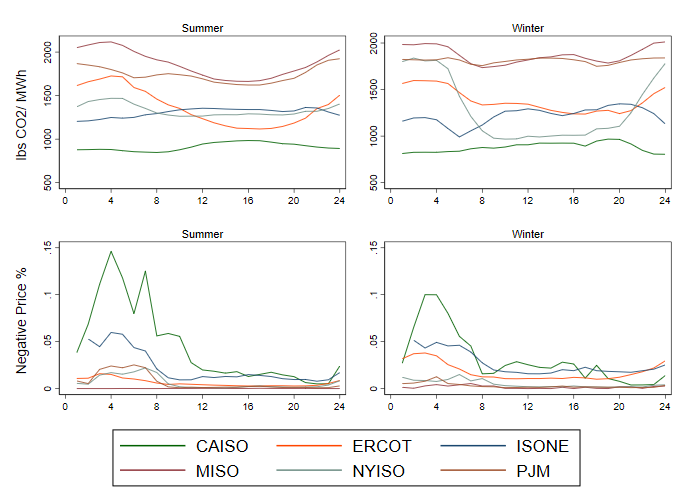
\includegraphics[width=0.75\textwidth]{moer_np_season.png}
\end{center}
\vspace{-15pt}
\footnotesize
Estimates of marginal operating emissions rates by hour of day and season were extracted from the appendix of \citet{callaway_location_2018}. Figures in the second row plot the mean share of negative price hours by ISO for the same hours and seasons. %
\end{figure}


The third panel of Table~\ref{tab:Frequency-of-Negative} contains average marginal emissions rates for each ISO. These emissions rates vary across regions, but are still positive and large everywhere, even when weighted by the negative prices in each ISO-season-hour. Finally, we present the correlation between negative prices and marginal operating emissions rates in the last row of Table~\ref{tab:Frequency-of-Negative}. In four of the six electricity markets, negative prices are positively correlated with marginal operating emissions rates, suggesting that the \textit{external} social value of wind energy during these hours is at least as high as during other time periods.

Finally, Figure~\ref{fig:md_np_hmmy} presents estimates of the average marginal damages from electricity generation in monetary terms from \cite{holland_are_2016}. These numbers include damages from both local and global air pollution. These estimates suggest that marginal damages are equal to or larger than the nominal value of the PTC in most regions and hours when averaged over all days of the year.

\begin{figure}[ht]
\begin{center}
\caption{Marginal Emissions Damages by Hour of Day \label{fig:md_np_hmmy}}
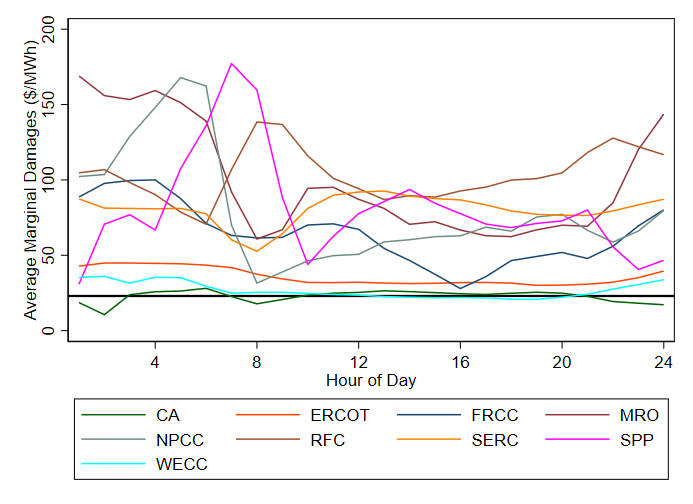
\includegraphics[width=0.75\textwidth]{md_np_hmmy.png}
\end{center}
\footnotesize Estimates of external marginal damages from electricity generation by hour of day and NERC region are taken from the replication materials for \citet{holland_are_2016}. The horizontal line is the nominal value of the PTC (\$23/MWh).
\end{figure}


\clearpage
\section{Cost-Effectiveness Details \label{Appendix:CostEffectiveness}}
\subsection{Profit Calculation Details \label{Appendix:Profitability-calculation-detail}}

Sections \ref{subsec:Extensive} and \ref{sec:costEffectiveness} approximate plant entry decisions using estimates of projected discounted profits under both subsidy regimes. These profit calculations require making assumptions about lifetime production, prices, operating costs, and discount rates. This appendix discusses each of these assumptions and presents additional sensitivity analysis.

The starting point for these calculations is two estimates of discounted lifetime profits for each plant given by:

\begin{align*}
\pi_i^{1603}&=\sum_{t=1}^{t=25} \left(\frac{p_{it}}{(1+r)^{t}}\right) Q_{it} - \frac{c_{it}}{(1+r)^{t}} -(1-s)F_i \\
\pi_i^{PTC}&=\sum_{t=1}^{t=25}\left(\frac{p_{it}}{(1+r)^t} + \frac{\phi_{it}}{(1+r^{tax})^t} \right) Q_{it} 
 + \frac{\frac{1}{2} \phi_{it}}{(1+r^{tax})^t} \Delta Q_{it}(\phi_{it})
 - \frac{c_{it}}{(1+r)^t} - F_i\label{eq:piPTC_app}
\end{align*}

\paragraph*{Time Horizon}
Plants are assumed to remain in service for 25 years, and right-censored prices and quantities are imputed with the observed (real) averages for each plant.

\paragraph*{Output Prices}

Plant-specific output prices ($p_{it}$) are computed using resale revenues reported on EIA Form 923, power purchase agreements from AWEA and BNEF, and estimated revenue from the sale of RECs.

Form EIA-923 began collecting annual resale revenue and quantity for each plant in 2011. The EIA refers to these data as ``resale,'' since the purchasing entity resells the power to end-use consumers. We infer average resale prices by dividing revenue by quantity and use this price for plants that sell all of their electricity for resale. For plants that report retail sales, we use average annual retail price information at the state level from Survey \href{https://www.eia.gov/electricity/data/eia861m/index.html}{EIA 861M}. In cases where firms report both types of sale, we construct a weighted average price. We exclude plants that are missing data on sales for resale and retail sales. We assume real prices remain at their current levels in future periods.

We also incorporate PPA data from AWEA and BNEF.  Both sources report multiple prices for some plants, and we use the median price for each plant from each source. We then take the maximum price derived from EIA resale data, AWEA resale data, and BNEF data as the price firms receive for their output in the electricity market.

Finally, we include estimated marginal revenue from the sale of RECs under state-level renewable portfolio standards using data from Marex Spectron and Lawrence Berkeley National Laboratory. As of 2017, 29 states and Washington D.C. had enacted RPSs. Wind farms generate certificates for each unit of production, which they then sell to utilities subject to the RPSs. Unfortunately, these payments are not observed in the EIA data.

We construct estimates of the RPS payments available to wind farms in a given state-month using bid-ask data on RECs trades from all active state RECs markets collected by Marex Spectron through May 2015. To account for the fact that some states allow covered non-renewable entities to obtain credits from qualifying renewable generators outside the state, we combine these state level prices with annual estimates of cross-state REC compliance flows from Lawrence Berkeley National Lab.\footnote{More information on this project tracking cross-state RECs at \href{https://emp.lbl.gov/projects/renewables-portfolio}{https://emp.lbl.gov/projects/renewables-portfolio}.} This expected REC payment is added to the average resale price to get marginal revenue each period. 

\paragraph*{Output Quantities}
Output under the 1603 ($Q_{it}$) is calculated based on the observed capacity factor. Output under the PTC, $Q_{it} + \Delta Q_{it}(\phi_{it})$, is constructed by increasing observed capacity factor for each plant by 3.3 \unskip percentage points (reflecting the average of our preferred IV and matching results) for the first ten years of operation.

\paragraph*{O\&M Costs}
Plant-specific operations and maintenance costs ($c_{it}$) are unobserved, so we use \$29/kW/year (in 2018 dollars) for all plants based on \cite{wiser_2018_2019}.

\paragraph*{PTC Subsidy and Costs}
Under the PTC, firms receive $\phi_{it} = \$23$ additional dollars per MWh of output for first ten years of operation in the form of tax credits. Plants receive the full subsidy on inframarginal output that is generated under the 1603 ($Q_{it}$).

For additional electricity generated under the PTC, $\Delta Q_{it}(\phi_{it})$, O\&M costs are likely to be higher on the margin than on average. Lacking plant-specific O\&M costs, we assume that plants only receive half of the PTC subsidy value for marginal units. This is equivalent to assuming linear marginal costs for producing this marginal output.

\paragraph*{Fixed Costs}
Fixed investment costs ($F_i$) are obtained by dividing the observed 1603 grant award amount from Treasury by the fraction of investment costs covered by the program ($s=0.3$).

\paragraph*{Inflation Adjustment}
We put all revenues and costs in 2014 dollars. The PTC is indexed to inflation, so we use the 2014 value of \$23 per MWh for all PTC revenues. We observe other output prices (resale prices, PPAs, and RECs) and fixed costs ($F_i$) at different points in time for different projects. To put these prices in 2014 dollars, we follow the PTC inflation adjustment by using the GDP implicit price deflator from the U.S. Bureau of Economic Analysis.

\paragraph*{Discounting}
Output prices ($p_{it}$) and O\&M costs ($c_{it}$) are discounted at an assumed five percent real interest rate ($r$). The PTC subsidy ($\phi_{it}$) is discounted at a higher rate to account for the need to monetize tax credits discussed in Sections \ref{subsec:RenewablePolicies} and \ref{subsec:Extensive}. We use an eight percent interest rate ($r^{tax}$) because it is the modal tax equity yield over 2009-2012 presented in \citet{bolinger_analysis_2014}. We use the maximum observed tax equity yield of 10.5 percent for sensitivity analysis in Appendix \ref{Appendix:1603eval}.

\paragraph*{Accelerated Depreciation}
Wind farms were eligible for accelerated depreciation of fixed investment costs during the sample period. This can be viewed as an additional subsidy that may affect plant profitability. In addition, the value of accelerated depreciation depends on the subsidy firms choose: for 1603 recipients, the cost basis for depreciation is reduced by half the grant amount. This means that firms can depreciate 85 percent of the fixed cost under the 1603 versus 100 percent under the PTC.

While our focus is on the economic profits of wind farms rather than their financial structure and tax payments, the details of accelerated depreciation could affect plant profitability, plant subsidy choice, and government expenditures. To account for this, we compute the subsidy value of accelerated depreciation relative to straight line depreciation for each subsidy case. For accelerated depreciation, we first account for 50 percent bonus depreciation and then use the 5-year MACRS depreciation schedule from Table A-1 of the 2012 IRS Publication 946 for the remaining cost basis. For straight line depreciation, we depreciate the investment cost over the lifetime of production (assumed to be 25 years) and assume zero scrap value. We use the appropriate cost basis (85 percent or 100 percent of the investment cost) depending on the policy case. Depreciation flows are translated into dollars using a marginal tax rate of 35 percent and then converted to net present value using the assumed discount rate of five percent. Finally, we compute the subsidy value of accelerated depreciation by taking the difference between the depreciation ``revenues'' under these two schedules and adding that difference to plant profits. We also add that amount to the public expenditure to reflect the difference in tax receipts under the two subsidies.

\subsection{Section 1603 Program Evaluation \label{Appendix:1603eval}}

Table~\ref{tab:policyeval} summarizes these two constructed profit measures for 1603 grant recipients.\footnote{This sample differs slightly from the sample used in Section \ref{sec:Empirical-Strategy} because we exclude plants with no price data and include plants who were omitted from the regression analysis due to missing wind speed data.} The first two columns of the table report predicted lifetime output along with the total subsidy paid to 1603 claimants, both discounted using a five percent real interest rate.\footnote{Total government payments include accelerated depreciation benefits under each subsidy.} The third column presents the ratio of total subsidy to total output, which can be interpreted as the public LCOE. The final three columns present predicted output, subsidy, and public LCOE for these projects had they claimed the PTC instead of the 1603 grant. Plants are assigned to one of three groups: an always profitable group ($\pi^{1603}>0$ \& $\pi^{PTC}>0$), a marginal group ($\pi^{1603}>0$ \& $\pi^{PTC}<0$), and a never profitable group ($\pi^{1603}<0$ \& $\pi^{PTC}<0$).

Estimating the full effect of the 1603 program requires taking a stand on the counterfactual entry status of the never-profitable group. If these plants are in fact marginal, and would not have entered without the 1603 grant program, the 1603 program increased lifetime wind production by 85million MWh (14 \unskip percent) while increasing the average public LCOE by $\$ 2.26 $/MWh (8 \unskip percent). If instead the never-profitable plants would have entered in either case, the 1603 grant program screened in just 15million MWh of production (in discounted terms) at the 6marginal plants. At the same time, production at inframarginal plants declined. Under this assumption, our preferred assumption, total wind output would have been slightly \emph{higher} without the 1603 program (by 25million MWh, or 4percent). This would also imply that the 1603 grant increased the average public LCOE by $\$ 2.04 $/MWh (7 \unskip percent).

\begin{table}[H]
\caption{Estimated Subsidy by Group\label{tab:policyeval}}
\vspace{-15pt}
\begin{center}
\footnotesize
\newcolumntype{Y}{>{\raggedleft\arraybackslash}X}
\begin{tabularx} {\textwidth} {@{} l Y Y Y Y Y Y Y Y Y Y Y Y Y Y Y Y@{}} \\
\toprule
& & \multicolumn{3}{c}{1603} & \multicolumn{3}{c}{PTC} \\
\cmidrule(l{.75em}){3-5} \cmidrule(l{.75em}){6-8}
Group & N & Output (MMWh) & Subsidy (\textdollar M) & Subsidy (\textdollar/MWh) & Output (MMWh) & Subsidy (\textdollar M) & Subsidy (\textdollar/MWh) \\
\midrule
Always Profitable&176&562&17,564&31.24&596&17,674&29.67 \\
Marginal&6&15&674&43.58&17&599&35.97 \\
Never Profitable&29&103&3,488&34.00&109&3,401&31.07 \\
\bottomrule
\addlinespace[.75ex]
\end{tabularx}
\par
\normalsize
%\scriptsize{\emph{Source: }#}
\end{center}

\footnotesize
Estimated electricity generation and subsidy for 1603 recipients, divided into three groups depending on their estimated profitability under the 1603 grant and the PTC. Output and Subsidy are in net present value terms, and Subsidy per MWh is constructed by taking the ratio of the sum of discounted subsidy expenditures to the sum of discounted electricity generation as in the definition of the LCOE. The first set of numbers correspond to outcomes under the subsidy they chose. The second set presents a counterfactual for the subsidy they did not choose.
\end{table}

Table \ref{tab:policyeval_highrtax} summarizes the results of the profitability calculation when using the maximum observed tax equity yield of 10.5 percent for $r^{tax}$ instead of the median yield of 8 percent. Under this alternative assumption, the number of always profitable plants decreases from 176 \unskip to 175\unskip, while the number of marginal plants increases from 6 \unskip to 7\unskip. As above, estimating the full effect of the 1603 program requires taking a stand on the counterfactual entry status of the never-profitable group. Under the assumption that never-profitable plants are in fact marginal, the 1603 program increased lifetime wind production by 88million MWh (15 \unskip percent) and increased the public LCOE by $\$ 2.28 $/MWh (8 \unskip percent). If instead the never-profitable plants would have entered in either case, the 1603 grant increased the average public LCOE by $\$ 2.06 $/MWh (7 \unskip percent).

\begin{table}[H]
\caption{Estimated Subsidy by Group using $r^{tax} = 10.5\%$\label{tab:policyeval_highrtax}}
\vspace{-15pt}
\begin{center}
\footnotesize
\newcolumntype{Y}{>{\raggedleft\arraybackslash}X}
\begin{tabularx} {\textwidth} {@{} l Y Y Y Y Y Y Y Y Y Y Y Y Y Y Y Y@{}} \\
\toprule
& & \multicolumn{3}{c}{1603} & \multicolumn{3}{c}{PTC} \\
\cmidrule(l{.75em}){3-5} \cmidrule(l{.75em}){6-8}
Group & N & Output (MMWh) & Subsidy (\textdollar M) & Subsidy (\textdollar/MWh) & Output (MMWh) & Subsidy (\textdollar M) & Subsidy (\textdollar/MWh) \\
\midrule
Always Profitable&175&559&17,441&31.19&592&17,560&29.65 \\
Marginal&7&19&797&42.83&20&713&35.59 \\
Never Profitable&29&103&3,488&34.00&109&3,401&31.07 \\
\bottomrule
\addlinespace[.75ex]
\end{tabularx}
\par
\normalsize
%\scriptsize{\emph{Source: }#}
\end{center}

\footnotesize
Estimated electricity generation and subsidy for 1603 recipients, divided into three groups depending on their estimated profitability under the 1603 grant and the PTC. Output and Subsidy are in net present value terms, and Subsidy per MWh is constructed by taking the ratio of the sum of discounted subsidy expenditures to the sum of discounted electricity generation as in the definition of the LCOE. The first set of numbers correspond to outcomes under the subsidy they chose. The second set presents a counterfactual for the subsidy they did not choose.
\end{table}


\subsection{Modifications for Cost-Effectiveness Analysis\label{Appendix:CostEffectiveness-calculation-detail}}

For the cost-effectiveness analysis in Section \ref{sec:costEffectiveness}, we simplify our profitability calculations to focus on the core economic tradeoffs of input and output subsidies. The most prominent changes are summarized in the text, and the rest are summarized below.

\paragraph*{Fixed Cost Estimation for PTC Recipients}
Extending this analysis to PTC plants requires information on the investment costs of these plants. For 1603 plants, investment costs are observed because they are subsidized. For PTC plants, no such government information is available. To fill this gap, we collect plant-level investment costs from a variety of sources: SNL Energy, BNEF, state tax filings and press releases. Of the 97 \unskip sample PTC plants entering between 2009 and 2012, we could not find cost information for 65 \unskip of these plants. 

We predict missing costs using a linear regression of costs onto plant characheristics for the plants whose costs we do observe. The sample is restricted so plants coming online within one year of the policy period (2008 - 2013). Cost are available for 284 \unskip  plants during this period, 79 \unskip of which claimed the PTC. Table \ref{tab:cost_prediction} presents the results. The dependent variable in each regression in the cost per unit of capacity (million \$/MW), and all models include plant vintage fixed effects. Model 1 shows that 1603 plants cost \$70,000 more per MW of capacity within cohort, although this estimate is not significantly different from zero. After controlling for plant size (model 2) and turbine firm and size (model 3), there is effectively no difference in costs between PTC and 1603 plants. After including state fixed effects in column 4, the root mean square error is \$270,000, which is approximately ten percent of the sample average cost. This final model is used for imputing missing plant costs in Section \ref{sec:costEffectiveness}.


\begin{table}[H]
\caption{Fixed Cost Estimation \label{tab:cost_prediction}}
\begin{center}
{
\def\sym#1{\ifmmode^{#1}\else\(^{#1}\)\fi}
\begin{tabular}{l*{4}{c}}
\toprule
                &\multicolumn{1}{c}{(1)}         &\multicolumn{1}{c}{(2)}         &\multicolumn{1}{c}{(3)}         &\multicolumn{1}{c}{(4)}         \\
\midrule
1603 Grant      &    0.076         &  0.00056         &    0.022         &   0.0074         \\
                &  (0.058)         &  (0.057)         &  (0.055)         &  (0.059)         \\
\addlinespace
Log(Capacity)   &                  &   -0.096\sym{***}&    -0.11\sym{***}&   -0.089\sym{***}\\
                &                  &  (0.021)         &  (0.019)         &  (0.021)         \\
\addlinespace
Turbine Capacity&                  &                  &     0.12\sym{**} &    0.042         \\
                &                  &                  &  (0.061)         &  (0.075)         \\
\midrule
Manufacturer FE &                  &                  &        Y         &        Y         \\
State FE        &                  &                  &                  &        Y         \\
adj R-sq.       &    0.085         &     0.17         &     0.39         &     0.49         \\
N               &      284         &      284         &      284         &      284         \\
rmse            &     0.35         &     0.34         &     0.29         &     0.27         \\
\bottomrule
\end{tabular}
}

\end{center}
\footnotesize
The dependent variable in each regression is the upfront investment cost in million \$/MW. Sample restricted to plants entering 2008-2013 with non-missing investment costs. All models contain cohort (year of entry) dummies. Robust standard errors reported in parentheses.
\end{table}

\paragraph*{Omit Accelerated Depreciation}
We focus on economic profits and omit the subsidy value of accelerated depreciation described above.

\paragraph*{Discounting}
We abstract from the tax credit nature of the PTC and discount PTC revenues at the same rate as electricity revenues (i.e., 5 percent).


\subsection{Relaxing the Correlations between Electricity Price and Productivity \label{Appendix:PriceCorrelation}}

In Section \ref{sec:costEffectiveness}, we demonstrated that, due to a negative correlation between output prices and investment productivity, output subsidies were more cost-effective than investment subsidies. In this section, we provide an alternative illustration of this point, by recomputing the public supply curve for wind energy with that correlation removed. 

Figure \ref{fig:pub_lcoe_meanprice} presents an alternative version of Figure \ref{fig:pub_lcoe} based on a hypothetical scenario in which all plants receive the sample average price for their electricity output. In this hypothetical scenario, the correlation between electricity price and investment productivity is zero, in contrast to the negative correlation observed in the data as shown in Figure \ref{fig:price_vs_capprod_1603}. Under this scenario, if plant production is held is fixed, investment subsidies are uniformly cheaper than output subsidies, consistent with \citet{parish_relative_1982}. When output is allowed to respond to output incentives, the two are similarly cost-effective, particularly at high subsidy levels. 

\begin{figure}[htb]
  \caption{Hypothetical Public LCOE vs Electricity Generation by Subsidy Type \label{fig:pub_lcoe_meanprice}}
  \begin{center}%\centering
  \begin{subfigure}[b]{0.495\textwidth}
    \caption{1603 Recipients \label{fig:pub_lcoe_1603_meanprice}}
    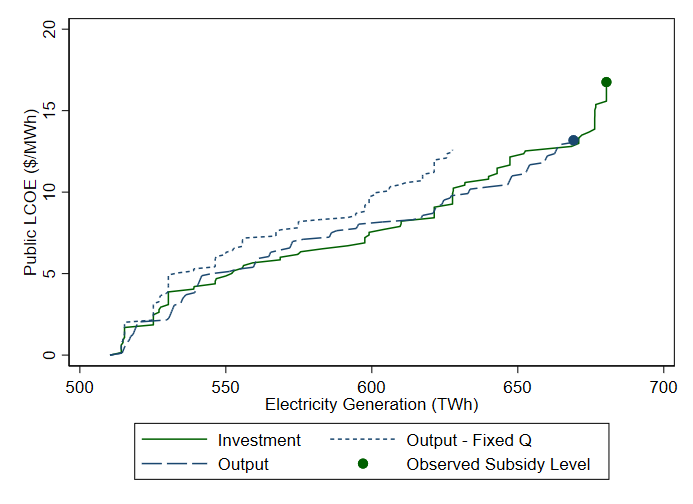
\includegraphics[width=\textwidth]{plcoe_plot_1603plants_meanprice.png}
  \end{subfigure} \hfill
  \begin{subfigure}[b]{0.495\textwidth}
    \caption{All Plants \label{fig:pub_lcoe_all_meanprice}}
    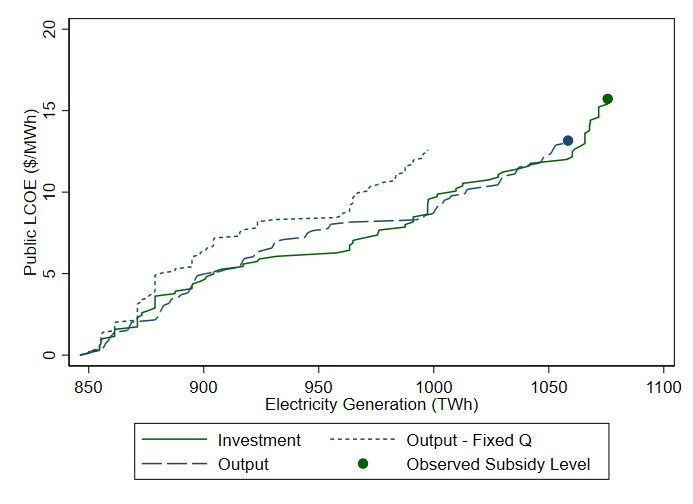
\includegraphics[width=\textwidth]{plcoe_plot_all_meanprice.png}
  \end{subfigure}
  \end{center}
  \vspace{-15pt}
  \footnotesize
  This is an alternative version of Figure \ref{fig:pub_lcoe} based on a hypothetical scenario in which all plants receive the sample average price for their electricity output. Each line plots the average public subsidy per unit of wind generation (LCOE) as a function of the total amount of wind generation subsidized. These are constructed by gradually increasing the subsidy from zero to the observed subsidy rates of the 1603 grant (investment) and PTC (output) subsidies. For output subsidy levels inframarginal to the PTC, we scale the estimated impact of the PTC on production linearly. For comparison, the ``Output - Fixed Q'' line plots the LCOE under the assumption that output is subsidized, but that this increase in marginal incentives does not affect plant productivity, conditional on operating. Panel (a) restricts the set of potential entrants to those selecting the 1603 grant, while panel (b) includes all wind farms entering between 2009 and 2012. In both figures, plants which are not marginal to either subsidy over the relevant range are assumed to always enter. The total output of these plants is reflected in the X-intercept of each figure. 
\end{figure}



\clearpage
\section{Additional Tables and Figures}

\subsection{Summary Stats}

\begin{table}[H]
\caption{Summary Statistics by Entry Date \label{tab:Summary-Statistics}}
\vspace{-15pt}
\begin{center}
\footnotesize
\newcolumntype{Y}{>{\raggedleft\arraybackslash}X}
\begin{tabularx} {\textwidth} {@{} l Y Y Y Y Y Y Y Y Y Y Y Y Y Y Y Y@{}} \\
\toprule
Year & Plants (all) & Plants (sample) & Plants (1603) & IOU or IPP & Regulated & Capacity & Turbine Size & Wind Speed & Capacity Factor \\
\midrule
2002&12&9&0&0.75&0.33&48.46&1.21&17.97&29.83 \\
2003&36&29&0&0.86&0.08&44.93&1.33&18.64&31.34 \\
2004&14&9&0&0.86&0.21&26.89&1.49&17.69&32.33 \\
2005&23&17&0&0.74&0.17&92.38&1.50&18.59&35.38 \\
2006&44&36&0&0.93&0.14&43.08&1.44&17.86&34.91 \\
2007&52&44&0&0.94&0.12&105.65&1.77&18.48&35.74 \\
2008&95&69&0&0.95&0.15&84.74&1.80&17.89&34.48 \\
2009&103&77&65&0.84&0.17&91.70&1.81&17.65&31.85 \\
2010&62&49&44&0.89&0.08&67.50&1.76&17.02&32.12 \\
2011&91&64&62&0.80&0.13&74.47&1.92&17.22&31.15 \\
2012&149&109&74&0.93&0.11&87.77&1.99&17.22&34.33 \\
2013&11&0&0&0.73&0.09&71.64&1.75&18.14&34.86 \\
2014&38&0&0&0.84&0.16&92.59&1.82&18.59&31.30 \\
\bottomrule
\addlinespace[.75ex]
\end{tabularx}
\par
\normalsize
%\scriptsize{\emph{Source: }#}
\end{center}

\footnotesize
Each row contains summary statistics for the set of wind farms in our sample that were placed into service in that year. Plants (all) is the number of wind farms placed into service in that year, Plants (sample) is the number in our restricted sample (see text and Appendix~\ref{sec:Data_Appendix}), and Plants (1603) is the number of Section 1603 grant recipients. All remaining columns are constructed using 2014 data from EIA Forms 860 and 923 except for Capacity and Turbine Size, which are constructed using the first values reported to the EIA. IOU or IPP is the share of wind farms that are owned by an investor-owned utility or independent power producer. Regulated is the share of wind farms that are regulated. Capacity is the average total nameplate capacity in MW. Turbine Size is the average turbine capacity in MW. Wind Speed is the average annual wind speed in miles per hour for each wind farm as reported to the EIA. Capacity Factor is the average of net electricity generation divided by capacity.
\end{table}

\clearpage

\begin{sidewaysfigure}[h] \centering
	\caption{New Wind Farms by Subsidy (2009-2012)\label{map:2009to2012}}
	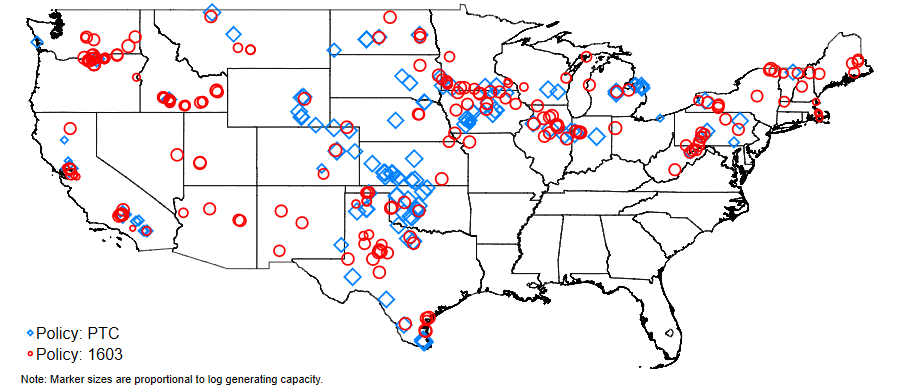
\includegraphics[width=\textwidth]{map_2009to2012.png}
\end{sidewaysfigure}

\begin{sidewaysfigure}[h] \centering
	\caption{New Wind Farms by Subsidy (2008-2009)\label{map:2008to2009}}
	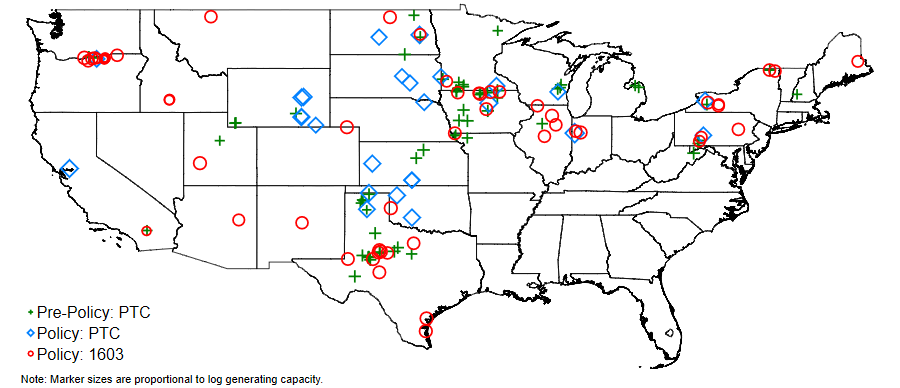
\includegraphics[width=\textwidth]{map_2008to2009.png}
\end{sidewaysfigure}

\subsection{Additional Results}

\begin{table}[H]
\caption{IV Results Sensitivity: Linear RD \label{tab:rdd_cf_linear}}
\begin{center}{\footnotesize{}{
\def\sym#1{\ifmmode^{#1}\else\(^{#1}\)\fi}
\begin{tabular}{l*{6}{c}}
\toprule
                &\multicolumn{1}{c}{(1)}         &\multicolumn{1}{c}{(2)}         &\multicolumn{1}{c}{(3)}         &\multicolumn{1}{c}{(4)}         &\multicolumn{1}{c}{(5)}         &\multicolumn{1}{c}{(6)}         \\
\midrule
1603 Grant      &   -3.697\sym{***}&   -2.893\sym{**} &   -3.156\sym{***}&   -6.376\sym{**} &   -4.774\sym{**} &   -1.346         \\
                &  (1.351)         &  (1.238)         &  (1.170)         &  (2.520)         &  (2.241)         &  (2.244)         \\
\addlinespace
Regulated       &                  &   -1.371         &   -5.446\sym{***}&                  &   -2.305         &   -5.980\sym{***}\\
                &                  &  (1.685)         &  (1.970)         &                  &  (1.881)         &  (1.943)         \\
\addlinespace
PPA             &                  &   -0.600         &   -2.618\sym{***}&                  &   -0.465         &   -2.704\sym{***}\\
                &                  &  (1.056)         &  (0.925)         &                  &  (1.063)         &  (0.952)         \\
\addlinespace
IPP             &                  &   -1.408         &   -2.514\sym{*}  &                  &   -1.883         &   -3.105\sym{**} \\
                &                  &  (1.305)         &  (1.307)         &                  &  (1.337)         &  (1.364)         \\
\addlinespace
Potential Capacity Factor&                  &    0.503\sym{***}&    0.553\sym{***}&                  &    0.503\sym{***}&    0.560\sym{***}\\
                &                  & (0.0368)         & (0.0386)         &                  & (0.0383)         & (0.0362)         \\
\addlinespace
Var(Wind Speed) &                  &   0.0637         &   -0.432\sym{***}&                  &  0.00692         &   -0.433\sym{***}\\
                &                  &  (0.155)         &  (0.107)         &                  &  (0.160)         &  (0.108)         \\
\addlinespace
log(Capacity)   &                  &   -0.605         &    0.580         &                  &   -0.643         &    0.600         \\
                &                  &  (0.430)         &  (0.470)         &                  &  (0.423)         &  (0.478)         \\
\midrule
Regression Type &     2SLS         &     2SLS         &     2SLS         &     2SLS         &     2SLS         &     2SLS         \\
Controls        &        N         &        Y         &        Y         &        N         &        Y         &        Y         \\
State FE        &        N         &        N         &        Y         &        N         &        N         &        Y         \\
Piecewise Trend &        N         &        N         &        N         &        Y         &        Y         &        Y         \\
N               &     8752         &     8752         &     8752         &     8752         &     8752         &     8752         \\
First-stage F-stat.&      148         &      169         &      113         &       38         &       32         &       22         \\
\bottomrule
\end{tabular}
}
}\end{center}
\footnotesize
Data include a balanced panel of monthly observations from 2010 to 2014 for all wind farms. The first three columns replicate the IV results in Table~\ref{tab:rdd_cf}. For columns 4 - 6, distance to the policy cutoff, and that distance interacted with a post-policy indicator are included as controls. All models contain year-month dummies. Standard errors, clustered at the plant level, are reported in parentheses.
\end{table}


\begin{table}[h]
\caption{Matching Results Sensitivity: Matching on Potential Capacity Factor \label{tab:matching_group_ptnlcf}}
\begin{center}
{
\def\sym#1{\ifmmode^{#1}\else\(^{#1}\)\fi}
\begin{tabular}{l*{5}{c}}
\toprule
                    &\multicolumn{1}{c}{(1)}         &\multicolumn{1}{c}{(2)}         &\multicolumn{1}{c}{(3)}         &\multicolumn{1}{c}{(4)}         &\multicolumn{1}{c}{(5)}         \\
\midrule
1603 Grant          &      -2.942\sym{***}&      -3.884\sym{***}&      -3.120\sym{***}&      -2.712\sym{**} &      -2.780\sym{**} \\
                    &     (0.719)         &     (1.027)         &     (1.067)         &     (1.098)         &     (1.196)         \\
\midrule
Sample              &         All         &     Matched         &     Matched         &     Matched         &     Matched         \\
FEs                 &       State         &       State         &       Group         &     Group*Y         &   Group*Y*M         \\
R-sq.               &       0.615         &       0.633         &       0.655         &       0.669         &       0.789         \\
N                   &       21303         &       12885         &       12885         &       12885         &       12885         \\
\bottomrule
\end{tabular}
}

\end{center}
\footnotesize
The matched sample was constructed using coarsened exact matching on state, regulatory status, entity type, capacity, and potential capacity factor. All models include the controls listed in the IV models in Table~\ref{tab:rdd_cf}: log capacity, potential capacity factor, and wind speed variance, as well as dummies for whether the plant is regulated, whether it is an IPP, the presence of a PPA, and month of sample. All models also include cohort dummies. Standard errors, clustered at the plant level, are reported in parentheses.
\end{table}

\subsection{Additional Data on Power Plant Proposal and Completion}

\begin{figure}[h]
\caption{Share of Plants Ever Completed, Plotted by Year of Initial Expected Completion\label{fig:proposed_ever_completed}}
\vspace{-15pt}
\begin{center}
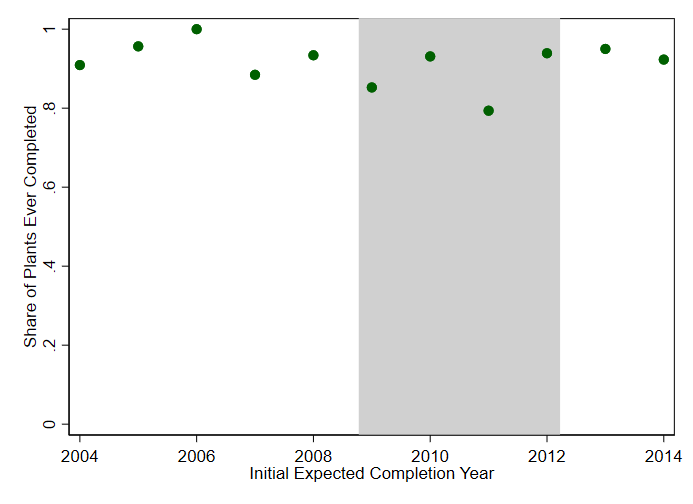
\includegraphics[width=0.75\linewidth]{proposal_data_ever_completed.png}
\end{center}
\vspace{-15pt}
\footnotesize
The initial expected completion year is the year the generator was first scheduled to start operation. Completion is determined based on when each plant entered into the EIA-860 operable data. Plots are based on the subset of plants that last appeared in the EIA-860 proposed data prior to 2016. Shading indicates the years during which new plants were eligible for the 1603 grant (2009 to 2012).
\end{figure}

\clearpage
%\begin{singlespace}
\bibliographystyle{jaere}
\bibliography{1603_all}
%\end{singlespace}

\end{document}

